% =====================================================================
% VERSION ENSAE, REDUCTION SFE (phase 3, 1er octobre 2026) : chapitre 1, risque cyber, DORA et cadre prudentiel.
% Copie a texte constant de chapitres/02b_cadre_cyber_dora.tex (lignes 1 a 682) puis chapitres/04_cadre_reglementaire.tex (en entier, devenu la section 1.6).
% Ne changent que les titres et les renvois repares, listes dans
% reduction/phase3.md.
% Lu par main_ensae.tex seul : ne jamais le faire lire par main_institut.tex,
% qui garde chapitres/.
% =====================================================================

% =====================================================================
% CHAPITRE 1 : RISQUE CYBER, RESILIENCE NUMERIQUE ET BESOIN DE CAPITAL.
%
% CE CHAPITRE SUIT LE PLAN ARRETE PAR KELIAN. Cinq sections, de la definition du risque a la
% problematique, sur le modele progressif du chapitre 1 de F. Dountio (ENSAE, 2026).
%
% CE QU'IL ABSORBE, ET C'EST LA DECISION DE STRUCTURE LA PLUS LOURDE DU FICHIER. Le plan met
% DORA en section 4 et la problematique en 5.3, or ces deux contenus vivent aujourd'hui dans
% 04_cadre_reglementaire.tex et 02_introduction.tex. SI CE CHAPITRE EST RETENU :
%   - 02_introduction.tex doit disparaitre ou se reduire a ce que 2b.5.3 ne reprend pas. Sa
%     section LUCY (sec:lucy) est reprise ici en section 3 et NE DOIT PAS figurer deux fois ;
%   - 04_cadre_reglementaire.tex doit se reduire a la seule articulation avec Solvabilite II,
%     le cadre DORA lui-meme passant ici. Son label chap:reglementaire doit survivre, cinq
%     chapitres le citent.
% Ne pas compiler le document avec ce chapitre ET les deux autres en l'etat : le lecteur lirait
% deux fois la meme lecture de marche et deux fois les cinq piliers.
%
% LES TROIS SOURCES DE CONTEXTE ET LEUR STATUT. Les valeurs 2026 de la cartographie France
% Assureurs, du barometre CESIN et de l'etude LUCY sont TRANSCRITES dans config.py sous
% CARTO_FA_2026, CESIN_2026 et LUCY_2026, au statut de CITATION EXTERNE NON RECALCULABLE. Le
% depot ne detient aucune de ces donnees d'origine : il ne peut que verifier la fidelite de la
% recopie, ce que font les scripts 63 (LUCY) et 103 (cartographie et barometre). Aucune n'entre
% dans une calibration et aucune ne porte un montant de capital. NE PAS ecrire une valeur de ces
% sources directement ici : elle echapperait au harnais, ce qui est la classe de defaut qui a
% produit les queues Bale et le Hill a 1,42.
%
% LES FIGURES SONT EXTRAITES DES RAPPORTS, comme les trois figures LUCY, et vivent dans
% memoire_cascade/figures_externes/, exception declaree du projet. Son README doit etre complete
% pour chaque figure ajoutee : provenance, page, recadrage. L'AUTORISATION DE REPRODUCTION EST
% ACQUISE POUR TOUTES : accordee par Hugo Rapior le 17 septembre pour les figures LUCY, puis
% etendue par lui le 19 septembre a la cartographie France Assureurs, au barometre CESIN et a la
% carte Avast. Ne pas rouvrir.
%
% AUCUNE FIGURE EN PLEINE PAGE. La macro de figure cle est interdite depuis le 15 septembre.
% Figures en ligne, 5 a 9 cm imprimes.
% =====================================================================

\chapter{Risque cyber, DORA et cadre prudentiel}
\label{chap:cadre-cyber-dora}
\label{part:contexte}



%======================================================================
\section{Pertes, propagation et dépendance}
\label{sec:risque-cyber}

\subsection{Définition et périmètre du risque cyber}
\label{subsec:definition-cyber}
% HARNAIS-HORS-SECTION: section de definitions, sans valeur chiffree issue d'un calcul du projet.

Le risque cyber désigne les pertes liées à une défaillance des systèmes d'information, malveillante
ou non, qui touche la confidentialité des données, leur intégrité ou la disponibilité des services.
L'\emph{incident} couvre tout événement qui affecte la sécurité d'un système, erreurs humaines et
pannes comprises, tandis que la \emph{cyberattaque} en désigne le sous-ensemble intentionnel, abouti
et à impact significatif \citep{cesin2026}. DORA retient la notion la plus large. Son champ, celui
de l'incident lié aux technologies de l'information et de la communication, couvre ainsi une mise à
jour défectueuse qui immobilise un système, même en l'absence de tout adversaire. Nous chiffrons le risque opérationnel d'origine informatique de l'entité, quelle que soit l'intention ; les pénalités et le risque des polices cyber qu'un assureur vend ne sont pas modélisés.

On distingue quatre familles d'incidents selon leurs conséquences financières. Le rançongiciel
coûte surtout par l'interruption d'activité qu'il provoque. La fuite de données coûte avec retard, par les notifications, les actions de groupe et les sanctions. Le déni de service produit
une perte d'exploitation bornée dans le temps, tandis que la défaillance d'un prestataire ou d'un
logiciel tiers atteint simultanément tous ses clients et produit, par construction, des sinistres
corrélés.

\subsection{Incidents individuels et chocs de cause commune}
\label{subsec:chocs-cause-commune}
% HARNAIS-HORS-SECTION: section conceptuelle, aucune valeur chiffree.

Les trois premières familles produisent des incidents que la mutualisation absorbe. La quatrième
produit une \emph{accumulation}, puisque la compromission d'un prestataire partagé frappe en même temps
des assurés qui n'ont d'autre lien que ce fournisseur. Le même passage de l'incident isolé au choc
commun se produit à l'intérieur d'une entité, niveau que nous modélisons. Les piliers
n'y cèdent pas indépendamment les uns des autres, car une gouvernance défaillante retarde la
détection des incidents et une dépendance mal maîtrisée à un prestataire crée une vulnérabilité que
les tests n'ont pas explorée.

La propagation a un sens. Un pilier dont la défaillance entraîne les autres n'appelle pas la même
remédiation qu'un pilier qui subit la leur, alors que les statistiques disponibles n'enregistrent
qu'une co-occurrence. Nous construisons au chapitre~\ref{chap:cascade} la propagation dirigée qui distingue ces deux situations, avant d'étudier au chapitre~\ref{ch:identifiabilite} ce que les données
permettent d'en identifier.

\section{Limites de l'assurabilité et de la capitalisation du risque cyber}
\label{sec:assurabilite-capital}

\subsection{Fréquence, sévérité et contrat d'assurance}
\label{subsec:frequence-severite-contrat}
% HARNAIS-HORS-SECTION: section de cadrage actuariel, aucune valeur chiffree du projet.

On décompose la charge annuelle d'un risque en un nombre d'événements et un coût par événement,
c'est-à-dire la fréquence et la sévérité. Les mêmes mesures ne réduisent pas les deux, la
sensibilisation des collaborateurs agissant sur la fréquence et une capacité de reprise sur la
sévérité. Nous appliquons cette décomposition à l'écart de capital entre états de conformité
(chapitre~\ref{chap:resultats}).

Le contrat d'assurance transforme la perte. La \emph{franchise} laisse à l'assuré la première
tranche du sinistre et la \emph{capacité} plafonne l'engagement de l'assureur, si bien qu'une
charge indemnisée et une perte brute ne se comparent ni en niveau ni en quantile. Sur des données
agrégées, une baisse de franchise et une aggravation de la menace produisent le même signal, à
savoir une charge indemnisée qui monte. On retrouve cette situation au
chapitre~\ref{ch:identifiabilite}, à l'échelle des piliers, et nous la traitons de la
même façon, en bornant ce que la donnée ne sépare pas.

\subsection{Conditions d'assurabilité et asymétrie d'information}
\label{subsec:dependance-accumulation}
% HARNAIS-HORS-SECTION: section de cadrage, aucune valeur chiffree du projet.

Le risque cyber met à l'épreuve les conditions de l'assurabilité. La défaillance d'un prestataire commun accroît la dépendance des pertes et limite la mutualisation. Une attaque ciblée reste incertaine pour la victime ; son caractère intentionnel ne supprime pas à lui seul l'aléa assurable. L'historique
manque en outre là où se joue la quantification. L'asymétrie d'information entre assureur et assuré sur
l'état réel du système d'information renforce enfin l'aléa moral et l'anti-sélection. DORA agit sur
ce dernier point, car le registre des accords avec les prestataires, la notification des incidents
majeurs et les tests de résilience rendent la maîtrise du risque observable. Une méthode qui traduit
cette maîtrise en capital pourra exploiter cette information.

\subsection{Rareté des données extrêmes et limite de l'historique français}
\label{subsec:donnees-extremes}
% HARNAIS-HORS-SCRIPT: le niveau reglementaire 99,5 % est pose par la directive ; le recul
% de 20 % des sinistres et les millesimes 2020-2022 viennent d'analyses de sinistralite
% europeennes citees en bibliographie, que le depot ne detient pas et ne recalcule pas.

Le capital de solvabilité est un quantile à $99{,}5\,\%$ de la charge annuelle, dépassé une année
sur deux cents. Il dépend donc des sinistres les plus lourds, pour lesquels la donnée française est
presque vide (section~\ref{sec:marche-cyber-francais}). Pour estimer une queue par dépassement de
seuil, on ne retient que les pertes au-dessus d'un montant élevé, et il faut un effectif suffisant
au-delà de ce seuil, ce que l'historique national n'offre pas. Une estimation sur cette base serait
instable et sous-estimerait le risque, faute d'avoir observé les pertes qui le déterminent. C'est
pourquoi nous calibrons la sévérité sur une base internationale (chapitre~\ref{chap:donnees}).

Cette rareté ne traduit pas une protection du marché français. Les sinistres cyber européens
ont certes reculé d'environ $20\,\%$ en $2024$, mais restent près d'un tiers au-dessus des exercices
$2020$ à $2022$ \citep{marsh2025}, et le marché britannique est décrit comme plus exposé aux
sinistres sévères \citep{dsit2025}.

\section{Marché français de la cyberassurance}
\label{sec:marche-cyber-francais}
% SOURCES-SCRIPTS: 63

L'étude LUCY de l'AMRAE, dont l'édition $2026$ couvre l'exercice $2025$, observe le marché français
sur $20\,996$ polices et $1\,251$ sinistres déclarés, recueillis auprès de douze courtiers et d'un
assureur \citep{amraeLucy2026}. La série, engagée en $2019$, compte sept exercices comparables. Nous
avons co-écrit l'analyse actuarielle de cette édition \citep{RapiorKaddouri2026}. Ses valeurs sont
reprises comme des citations externes, que nous ne pouvons pas recalculer, et n'entrent ni dans le
modèle ni dans le calcul d'un montant de capital.

La charge indemnisée s'élève à $83{,}2$~M\euro{} en $2025$ contre $54{,}5$ l'exercice précédent, soit
$+53\,\%$. Nette de franchise et plafonnée par la capacité, elle ne se compare pas à la perte brute
d'une entité, que nous modélisons. Entre $2024$ et $2025$, le nombre d'entreprises assurées croît de
$49\,\%$, mais les primes reculent de $3\,\%$. Le ratio sinistres sur primes remonte depuis
deux exercices, de $12\,\%$ en $2023$ à $27\,\%$, loin des $169\,\%$ de $2020$.

La hausse du ratio recouvre deux régimes opposés. En $2024$, les sinistres sont moins nombreux
($\times 0{,}73$) mais deux fois plus lourds ($\times 1{,}96$). En $2025$, ils sont presque
trois fois plus nombreux ($\times 2{,}79$) pour un coût moyen divisé par deux ($\times 0{,}55$). Seule la
décomposition de la charge en nombre et coût moyen sépare ces deux situations, qui n'appellent pas
les mêmes mesures.

La limite qui engage notre modélisation se situe dans la queue. Deux exercices sur sept ne comptent
aucun sinistre de la classe de 10 à 40~M\euro{}, et un exercice y enregistre
$135$~M\euro{}. En $2025$, cette classe représente $19$~M\euro{}, pour un seul sinistre au-delà de
$10$~M\euro{} (figure~\ref{fig:lucy-taille}). L'historique national s'arrête avant le haut de la distribution. 

\begin{figure}[H]
\centering
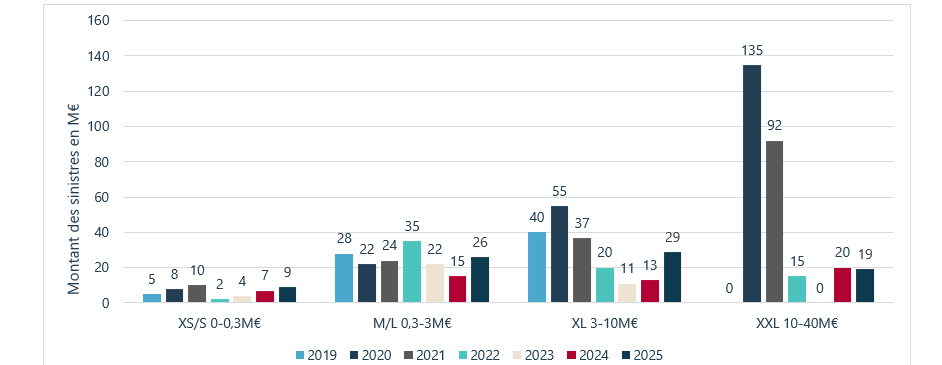
\includegraphics[width=0.80\textwidth]{figures_externes/lucy_taille_des_sinistres.png}
\caption{Charge indemnisée par classe de taille de sinistre, $2019$--$2025$. La classe la plus
haute est vide deux exercices sur sept : l'historique national s'arrête avant le haut de la
distribution.
Source : rapport LUCY 2026, Nexialog Consulting \citep{RapiorKaddouri2026}.}
\label{fig:lucy-taille}
\end{figure}

\section{Le règlement DORA}
\label{sec:dora}
% HARNAIS-HORS-SECTION: section reglementaire. Les seuls nombres sont des millesimes, des
% numeros d'articles et des references de textes, aucun ne provient d'un calcul du projet.

\subsection{Cadre réglementaire européen du cyber}
\label{subsec:cadre-reglementaire-europeen}
% HARNAIS-HORS-SECTION: section reglementaire. Les nombres sont la date d'entree en
% application, des millesimes et des numeros officiels de textes. Ce sont des donnees de droit.

Quatre textes européens encadrent le risque cyber. La directive NIS~2
\citep{NIS2Directive2022}, relative à la sécurité des réseaux et des systèmes d'information, impose
des exigences de sécurité et de notification aux entités essentielles et importantes. Elle rend
également l'organe de direction responsable des mesures de gestion du risque. Le règlement général
sur la protection des données \citep{RGPD2016} encadre les données personnelles, la directive sur la
résilience des entités critiques \citep{REC2022} la continuité des fonctions sociétales vitales. Le
règlement sur la cyberrésilience \citep{CRA2024} couvre enfin la sécurité des produits numériques.
Aucun n'est propre au secteur financier.

Le règlement DORA \citep{DORA2022} comble ce manque. Entré en application le $17$ janvier $2025$, il
s'adresse à une vingtaine de catégories d'entités financières, dont les entreprises d'assurance, et
leur demande de résister à l'incident, d'y réagir et de s'en rétablir. 

Nous ne modélisons que DORA, car il est le seul de ces textes à découper la résilience en piliers
dont la défaillance pourra se lire dans les incidents notifiés. Les cadres de l'intelligence
artificielle et de l'identité numérique ne sont pas traités. Le règlement sur la cyberrésilience,
applicable à partir de décembre~$2027$, agira sur la fréquence future des vulnérabilités. Notre calibration l'estime sur l'historique et ne la projette pas.

\subsection{Les cinq piliers de DORA}
\label{subsec:cinq-piliers-dora}
% HARNAIS-HORS-SECTION: section reglementaire. Les nombres sont les etiquettes P1 a P5, les
% numeros d'articles du reglement et les delais qu'il fixe. Ce sont des donnees de droit.

Le règlement organise la résilience en cinq domaines, notés P1 à P5, que nous appelons \emph{piliers}.
\begin{itemize}[leftmargin=1.4em,itemsep=2pt]
\item P1, gouvernance du risque lié aux technologies (articles~$5$ à~$16$) : responsabilité non
      délégable de l'organe de direction, cartographie des actifs et des dépendances critiques,
      contrôle interne continu.
\item P2, gestion, classification et notification des incidents (articles~$17$ à~$23$) : notification initiale dès que possible, sous quatre heures après classification majeure et au plus tard vingt-quatre heures après prise de connaissance. Si la classification intervient après ce délai, la notification suit sous quatre heures. Le rapport intermédiaire est dû sous soixante-douze heures après la notification initiale, le rapport final sous un mois après le rapport intermédiaire ou sa dernière mise à jour \citep{eu2025_301}.
\item P3, tests de résilience opérationnelle numérique (articles~$24$ à~$27$), dont des tests de
      pénétration guidés par la menace (TLPT), au moins tous les trois ans, pour les entités
      significatives (article~$26$).
\item P4, gestion du risque lié aux prestataires tiers (articles~$28$ à~$44$) : registre
      d'informations des contrats, clauses impératives de l'article~$30$, stratégie de sortie, et
      surveillance des prestataires critiques et prise en compte de leur chaîne de sous-traitance, sans limite générale au troisième rang.
\item P5, partage d'informations sur les cybermenaces (article~$45$), volontaire et encadré, le
      pilier le moins utilisable dans un calibrage actuariel.
\end{itemize}
Ces piliers ne sont pas indépendants, car un incident qui touche l'un dégrade la capacité de l'entité à tenir les autres (sous-section~\ref{subsec:chocs-cause-commune}). Nous formalisons cette dépendance au chapitre~\ref{chap:cascade}.

\subsection{Prestataires TIC, concentration et propagation du risque}
\label{subsec:risque-tiers-dora}
% SOURCES-SCRIPTS: 103

La sous-traitance informatique du secteur financier est concentrée sur un petit nombre de
fournisseurs, si bien qu'une défaillance chez l'un d'eux atteint de nombreuses entités sans faute de
leur part. DORA instaure pour cette raison une surveillance directe des prestataires critiques, ce qui
est nouveau dans l'architecture prudentielle européenne. Le premier bilan des notifications montre
le poids des prestataires. En $2025$, les sociétés de gestion ont adressé à l'Autorité des marchés
financiers $47$ notifications initiales, dont $31$ incidents majeurs confirmés, parmi lesquels $27$,
soit $87\,\%$, trouvent leur origine chez un prestataire \citep{amf2026incidents}.

Cette part dit d'où viennent les incidents ; elle ne fournit pas de probabilité de transfert entre piliers et ne calibre aucun paramètre du modèle. Les notifications initiales précèdent la confirmation du caractère majeur : l'écart avec les
incidents confirmés est celui d'un seuil de matérialité, et la collecte réglementaire ne retiendra que
les incidents au-dessus de ce seuil.

Pour la modélisation, l'exigence la plus utile est le registre d'informations. En recensant les
contrats TIC critiques et leurs chaînes de sous-traitance, il produit une donnée sur la concentration
technologique que l'évaluation interne des risques ne savait pas chiffrer. Il ne couvre que
la dépendance déclarée et ne dit rien de l'ordre dans lequel les défaillances s'enchaînent
(section~\ref{ch:livrable}). Les autorités de supervision ne publient pas de probabilité de
propagation entre piliers, si bien que les valeurs de propagation du modèle sont posées
à dire d'expert, puis bornées.

\section{Perception du risque et traitement prudentiel}
\label{sec:enjeu-prudentiel}

\subsection{Perception prospective selon France Assureurs et le CESIN}
\label{subsec:france-assureurs-cesin}
% SOURCES-SCRIPTS: 103 63

La cartographie prospective de France Assureurs classe le risque cyber au premier rang pour le
huitième exercice consécutif, avec un score de $4{,}1$ sur $5$ \citep{franceassureurs2026}. Ce score
a culminé à $4{,}48$ en $2022$ et revient à $4{,}10$ en $2026$ (figure~\ref{fig:carto-retro-rapport}).
Entre $2025$ et $2026$, il recule de $0{,}45$ point en fréquence anticipée et progresse de
$0{,}25$ point en sévérité.

D'après le baromètre du CESIN (Club des experts de la sécurité de l'information et du numérique), qui en donne le constat déclaré \citep{cesin2026}, $40\,\%$ des
entreprises interrogées ont subi au moins une cyberattaque significative en $2025$. L'hameçonnage
est cité par $55\,\%$ des entreprises attaquées, l'exploitation d'une faille par $41\,\%$ et l'attaque
indirecte par un tiers par $35\,\%$, part qui monte à $43\,\%$ dans les grandes entreprises. On
reconnaît là le pilier P4, vu par une source indépendante de ce travail.

Quatre entreprises attaquées sur cinq déclarent un impact sur leur activité, mais la sanction
d'une autorité ne concerne que $3\,\%$ des cas. Nous ne modélisons donc pas les pénalités : la
non-conformité coûte, dans le modèle, par les incidents qu'elle laisse passer. La déconnexion de l'entité par ses propres partenaires, citée dans $12\,\%$ des cas,
montre enfin que la dépendance joue dans les deux sens.

\begin{figure}[H]
\centering
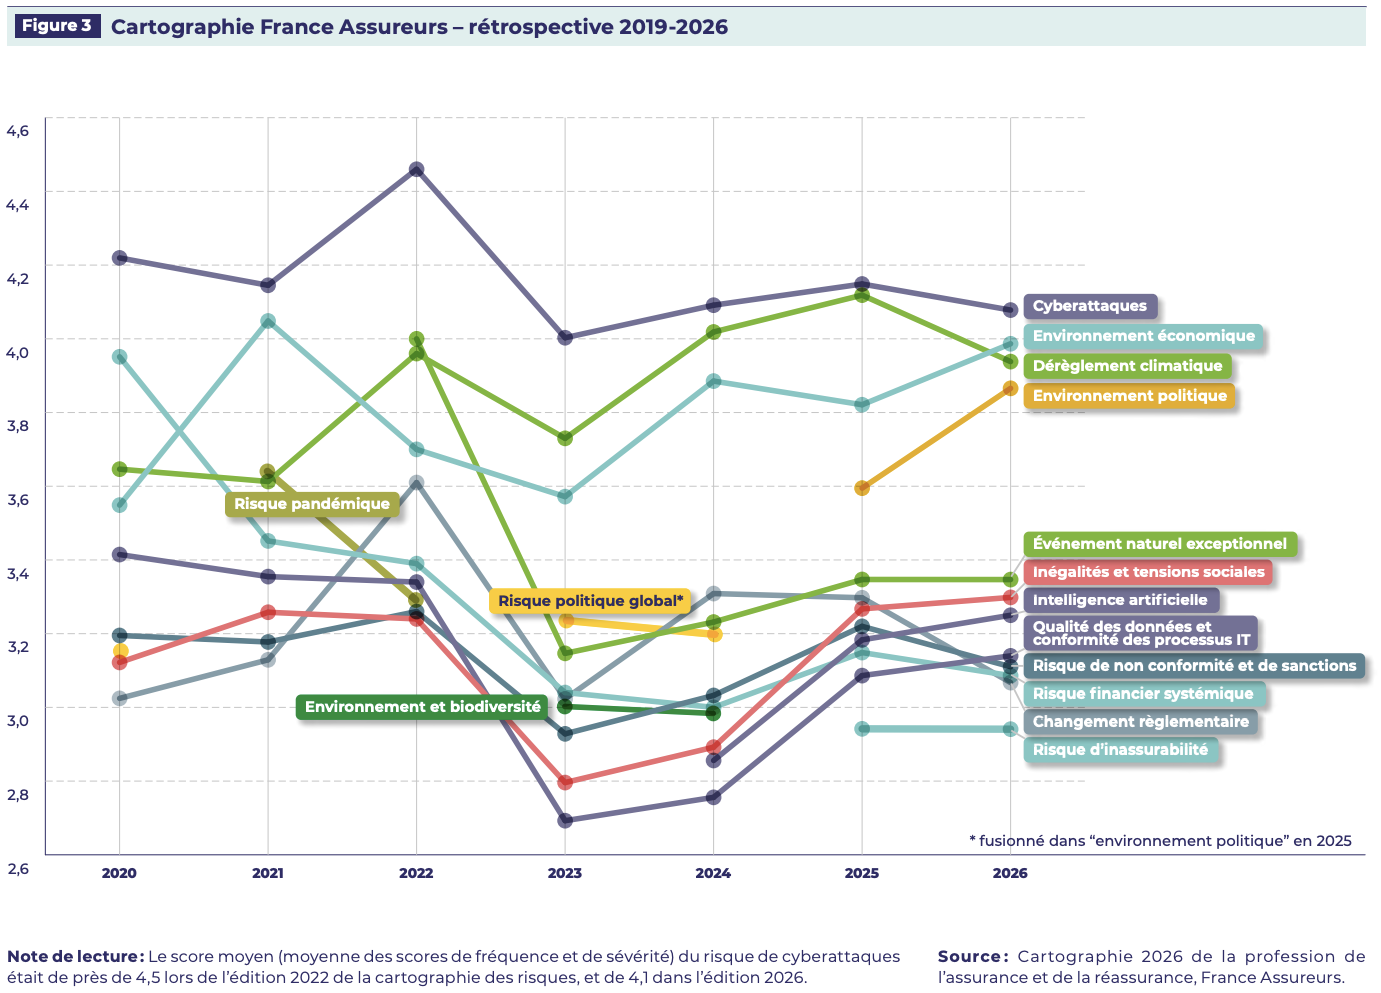
\includegraphics[width=0.72\textwidth]{figures_externes/carto_fa_2026_retrospective.png}
\caption{Trajectoire des scores de la cartographie prospective des risques de France Assureurs,
$2020$--$2026$. Le risque de cyberattaques reste au premier rang ; son score ne monte plus depuis
$2022$. Source : \citet{franceassureurs2026}.}
\label{fig:carto-retro-rapport}
\end{figure}

\subsection{Limites de Solvabilité II et de la Formule Standard}
\label{subsec:limites-formule-standard}
% HARNAIS-HORS-SECTION: section de cadrage prudentiel, aucune valeur chiffree du projet.

La Formule Standard de Solvabilité~II charge le risque opérationnel par un pourcentage de primes ou
de provisions techniques. Faute de
sous-module cyber, les assureurs sont renvoyés à leurs modèles internes et à leur évaluation interne
des risques (section~\ref{chap:reglementaire}).

Une copule, outil usuel, décrirait la loi jointe des pertes entre domaines, mais non l'ordre dans lequel un incident les atteint. Or deux matrices de dépendance transposées l'une de l'autre, que les statistiques
usuelles ne distinguent pas, conduisent en général à un capital différent
(chapitre~\ref{chap:cascade}).

\section{Cadre prudentiel et articulation avec DORA}
\label{chap:reglementaire}

% HARNAIS-HORS-SCRIPT: cadre reglementaire : numeros d'articles, delais de notification et seuils cites des textes (DORA, Solvabilite II, Bale). Ce sont des donnees de droit, pas des resultats.

Le risque opérationnel reçoit la même définition dans la banque et dans l'assurance. Il s'agit du
risque de perte résultant de l'inadaptation ou de la défaillance de procédures, de personnels et de
systèmes internes, ou d'événements extérieurs. Il comprend le risque juridique et exclut les risques
stratégique et de réputation.

Les modes de quantification ont cependant divergé. Le secteur bancaire a abandonné les
modèles internes de mesure avancée au profit d'une approche standardisée \citep{bcbs2017}, sans invalider l'approche
par distribution des pertes (LDA, \emph{Loss Distribution Approach}) comme outil de modélisation.
Nous en reprenons les deux marges, fréquence et sévérité, et remplaçons son agrégation par une
cascade dirigée. L'assurance conserve sous Solvabilité~II le choix entre la Formule Standard, des
paramètres propres à l'entreprise et un modèle interne, partiel ou global, approuvé par l'autorité de
contrôle.

Dans la Formule Standard, l'exigence pour risque opérationnel ($SCR_{Op}$) s'ajoute au capital de
solvabilité requis de base ($BSCR$), ajusté de la capacité d'absorption des pertes :
\begin{equation}
SCR = BSCR + Adj + SCR_{Op},
\qquad
SCR_{Op} = \min(0{,}3 \times BSCR,\ Op) + 0{,}25 \times Exp_{ul},
\label{reg:eq:scrop}
\end{equation}
où $Adj$ est l'ajustement pour la capacité d'absorption des pertes, $Exp_{ul}$ les frais annuels des contrats en unités de compte et $Op = \max(Op_{premiums}, Op_{provisions})$ applique des coefficients forfaitaires aux primes et
aux provisions. Cette forme est simplifiée, car l'article~204 du règlement délégué~2015/35 ajoute des
termes de croissance, de la forme $\max\!\left(0;\, 0{,}04 \times \Delta\!\right)$, qui pénalisent
les hausses de primes supérieures à $20\,\%$ d'un exercice à l'autre. Fondée sur des indicateurs de
volume, l'approche attribue la même exposition à deux assureurs de même volume, quelles que soient la
qualité de leur informatique et leur dépendance à des prestataires critiques. Le $SCR_{Op}$ réglementaire s'ajoute au BSCR sans diversification. Cela n'implique pas qu'un quantile ORSA supplémentaire doive être ajouté en entier : il faut éviter le double compte du risque informatique déjà couvert (\S\ref{sec:agregation-scr}).

Le $SCR_{Op}$ relève des exigences quantitatives (forfaitaires) de Solvabilité~II. Les exigences de gouvernance imposent l'évaluation
interne des risques et de la solvabilité (\emph{Own Risk and Solvency Assessment}, ORSA). Elle
confronte le profil de risque réel aux besoins de solvabilité et admet les scénarios stochastiques
que la Formule Standard ne produit pas. Notre modélisation se situe dans ce cadre. ORSA et DORA
partagent un objet, le risque opérationnel d'origine technologique, l'ORSA pour la continuité
financière, DORA pour la continuité opérationnelle. Nous partons d'états de conformité posés pour quantifier dans l'ORSA ce que celui-ci ne savait que décrire (chapitres~\ref{chap:multietats}
et~\ref{chap:resultats}).
